\documentclass{cours}
\usepackage{pgfplots}
\usepackage{multicol}
\usepackage{amssymb}
\usetikzlibrary {decorations.text}
\usepackage{mhchem}
\begin{document}

\setcounter{chapter}{16}
\chapter{Premier principe de la thermodynamique, échanges d'énergie}
\label{chap:premier_principe}

\section{Transformation thermodynamique}%
\label{sec:transformation_thermodynamique}
\begin{definition}
  Une transformation thermodynamique désigne le passage d'un état d'équilibre thermodynamique à une autre état d'équilibre.
\end{definition}

Une transformation peut être :
\begin{itemize}
  \item \textbf{isochore} : Le volume du système reste constant au cours de la transformation. 
  \item \textbf{isobare} : La pression du système reste constante au cours de la transformation. 
  \item \textbf{isotherme} : La température du système reste constante au cours de la transformation. 
  \item \textbf{monobar} : La pression du milieu extérieur reste constante au cours de la transformation. 
  \item \textbf{monotherme} : La température du milieu extérieur reste constante au cours de la transformation. 
  \item \textbf{adiabatique} : Il n'y a pas d'échange de chaleur avec le milieu extérieur.
\end{itemize}

\section{Travail des forces de pression}%
\label{sec:travail_des_forces_de_pression}
Lorsque le milieu extérieur exerce des forces de pression sur le système, il peut lui transférer de l'énergie par le biais du travail des forces de pression.

On considère le système constitué d'un cylindre fermé par un piston qui coulisse sans frottement et qui contient un gaz. On considère le système thermodynamique \{gaz+cylindre+piston\}.
On rappelle que le travail élémentaire fourni par une force $\vv{F}$ dont le point d'application se déplace de $\vv{\D l}$ est 
\begin{equation}
  \delta W = \vv{F}\cdot \vv{\D l}
\end{equation}

\begin{center}
  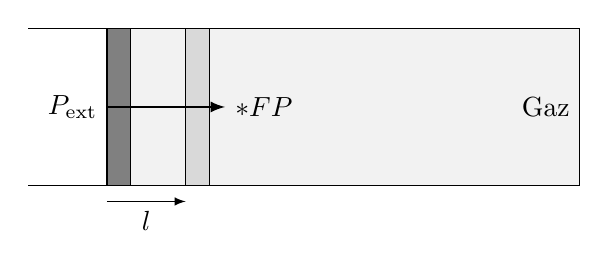
\begin{tikzpicture}
  %tikz thermo
    \fill[gray!10] (1,0) rectangle (7,2);
    \draw (0,0) -- ++(7,0) -- ++(0,2) -- ++(-7, 0);
    \draw[fill=gray] (1,0) rectangle ++(0.3, 2);
    \draw (1, 1) node[left]{$P_\text{ext}$};
    \draw (7,1) node[left]{Gaz};
    %\draw[-latex] (0, -1) -- ++(8,0) node[right]{$x$};
    \draw[fill=gray!30] (2,0) rectangle ++(0.3, 2);
    \draw[-latex] (1, -0.2) -- node[below] {$\vv{\D l}$} (2, -0.2);
    \draw[thick, -latex] (1, 1) -- ++(1.5, 0) node[right]{$\vv*{F}{P}$};
  \end{tikzpicture}
\end{center}
Dans ces conditions, le travail des forces de pression est:
\begin{equation}
  \delta W = \vv*{F}{P}\cdot \vv{\D l} = P_\text{ext}\underbrace{S\times\D l}_{-\D V} = -P_\text{ext}\D V
\end{equation}
où $\D V$ représente une variation élémentaire du volume du système. On peut généraliser cette expression à n'importe quelle déformation de n'importe quel système et écrire que le travail élémentaire fournie par les forces de pression à un système est toujours :
\begin{eqencadre}
  \delta W = -P_\text{ext} \D V
\end{eqencadre}
avec $P_\text{ext}$ la pression extérieure au système et $\D V$ une variation élémentaire du volume du système. 

On calcule le travail fourni par les forces de pression au cours d'une transformation qui amène le système d'un volume $V_1$ à un volume $V_2$ par l'intégrale :

\begin{eqencadre}
  W_{1\rightarrow 2} = \int_{V_1}^{V_2}-P_\text{ext}\D V
\end{eqencadre}

Pour une transformation isochore ($V=\text{constante}$) on aura $W=0$.  

On dit qu'une transformation est \textbf{quasistatique} lorsque tous les états intermédiaires de la transformation sont des états d'équilibre mécanique. Dans ce cas on aura à chaque instant de la transformation $P_\text{ext} = p$ où $p$ est la pression du système. Et on pourra écrire $\delta W = -p\D V$. 

Dans ce cas, on peut déterminer graphiquement le travail des forces de pression en représentant la transformation dans un diagramme de Watt $(P,V)$. 

\begin{center}
  \begin{tikzpicture}
  %tikz thermo
    \draw[-latex] (0,0) coordinate (O) -- (4, 0) node[right] {$V$ };
    \draw[-latex] (O) -- (0,3) node[left] {$p$ };
    \draw (0.5, 0) coordinate(A) node[below]{$V_A$};
    \draw (3.5, 0) coordinate(B) node[below]{$V_B$};
    \fill[gray!30] (A) -- ++(0, 0.5) to[bend left] ++(3,2) --(B);
    \draw[thick, postaction=decorate, decoration={markings, mark=at position 1.5cm with {\arrow{latex}}}] (A) ++(0,0.5) to[bend left] ++(3, 2) (B);
    \draw[dashed] (A) -- ++(0,0.5);
    \draw[dashed] (B) -- ++(0,2.5);
    \fill (A) ++(0, 0.5) circle(2pt);
    \fill (B) ++(0, 2.5) circle(2pt);
    \draw (2, 1.2) node{$W$ };
  \end{tikzpicture}
  \captionof{figure}{Transformation thermodynamique dans un diagramme de Watt}
\end{center}

Le travail fourni par les forces de pression lorsque le système passe de $V_A$ à $V_B$ est 
\begin{equation}
  W = \int_{V_A}^{V_B} -p(V) \D V = -\int_{V_A}^{V_B} p(V) \D V
\end{equation}

Il correspond à l'opposé de l'aire sous la courbe représentative de $p(V)$ entre $A$ et $B$. Si $V_B>V_A$ alors $W<0$.  

Une transformation \textbf{cyclique} est une transformation dont le point de départ et le point d'arrivée sont les mêmes.

\begin{center}
  \begin{tikzpicture}
  %tikz thermo
    \draw[-latex] (0,0) coordinate (O) -- (4, 0) node[right] {$V$ };
    \draw[-latex] (O) -- (0,3) node[left] {$p$ };
    \draw[preaction=fill, fill=gray!30]
          [thick, 
          postaction=decorate, 
          decoration={
            markings, 
            mark=at position 1.5cm with {\arrow{latex}},
            mark=at position 5.5cm with {\arrow{latex}}
          }
          ] (0.5, 1)coordinate (A) to[out=90, in=180] (2,2) node[above]{$(1)$} to[out=0, in=90](3.5,1) coordinate (B) to[out=-90, in=0](2,0.5) node[below]{$(2)$}to[out=180, in=-90] (0.5,1);
    \draw (2, 1.2) node{$W$ };
    \fill (A) circle(2pt) node[left]{$A$ };
    \fill (B) circle(2pt)node[right]{$B$ };
    \draw[dashed] (A) -- ++(0,-1) node[below]{$V_A$ };
    \draw[dashed] (B) -- ++(0,-1) node[below]{$V_B$ };
  \end{tikzpicture}
  \captionof{figure}{Transformation cyclique}
  \label{fig:transfo_cyclique}
\end{center}
Dans ce cas, le travail reçu par le système au cours d'un cycle est la somme du travail $W_1$ reçu pour aller de $A$ à $B$ par le chemin $(1)$ et du travail $W_2$ reçu pour aller de $B$ à $A$ par le chemin $(2)$  : 
\begin{equation}
  W = W_1 + W_2 = -\left(\int_{V_A}^{V_B}p_1(V) \D V - \int_{V_A}^{V_B}p_2(V)\D V\right)
\end{equation}
Le premier terme correspond à l'aire sous la courbe $(1)$ et le second terme correspond à l'aire sous la courbe $(2)$. La différence des deux correspond à l'aire du cycle.

Dans le cas de la figure~\ref{fig:transfo_cyclique} le cycle est parcouru dans le sens horaire et le travail reçu par le système sera négatif, on dit que le cycle est \textbf{moteur}, il fournit du travail au milieu extérieur.

Dans le cas où le cycle est parcouru dans le sens trigonométrique, le travail reçu par le système est positif et on dit que le cycle est \textbf{récepteur}.

Pour une transformation \textbf{monobare}, on aura
\begin{equation}
  W_\text{monobare}=\int-p_\text{ext}\D V = -p_\text{ext}\int\D V = -p_\text{ext}\Delta V
\end{equation}
où $\Delta V$ est la variation de volume du système au cours de la transformation.

\section{Transferts thermiques}%
\label{sec:transferts_thermiques}
\subsection{Types de transferts thermiques}%
\label{sub:types_de_transferts_thermiques}

Un système thermodynamique peut recevoir ou fournir de la chaleur (énergie thermique)
par trois mécanismes différents :
\begin{itemize}
  \item \textbf{La conduction} : La chaleur se propage au sein d'un matériau lorsque la température n'y est pas homogène. Par exemple une tige métallique chauffée à une extrémité s'échauffe à l'autre extrémité.
  \item \textbf{La convection} : La chaleur est transportée par la mise en mouvement de la matière (généralement un fluide). La convection peut être naturelle (le fluide se met en mouvement spontanément à cause d'une différence de température) ou forcée. Par exemple de l'eau chauffée par le bas dans une casserole transfert l'énergie thermiques aux couches supérieures par la mise en mouvement de l'eau chaude qui s'élève au dessus de l'eau plus froide.
  \item \textbf{Le rayonnement} : Un corps chauffé émet un rayonnement électromagnétique qui peut être capté par un autre corps. Il y a un transfert de chaleur. Par exemple un objet éclairé par le Soleil chauffe, le Soleil lui transfert de l'énergie thermique par rayonnement.
\end{itemize}

\subsection{Notion de thermostat}%
\label{sub:notion_de_thermostat}

Un thermostat est un système thermodynamique dont la température est constante. Il contient théoriquement une énergie interne infinie car il peut fournir de l'énergie thermique sans se refroidir.

En pratique un système se comporte comme un thermostat lorsque sa température varie très peu au cours d'une expérience donnée.

Par exemple, 
\begin{itemize}
  \item On plonge un petit caillou chauffé à \SI{100}{\celsius} dans un lac dont la température est de \SI{15}{\celsius}. La température d'équilibre du caillou sera de \SI{15}{\celsius} et la température du lac n'aura quasiment pas varié. Le lac peut être considéré comme un thermostat.
  \item L'hiver arrive et la température de l'atmosphère tombe à \SI{0}{\celsius}. La température du lac va finir par baisser à \SI{0}{\celsius}. Dans ce cas c'est l'atmosphère qui fera office de thermostat.
\end{itemize}

  \subsection{Transformations adiabatiques et isothermes}%
  \label{sub:transformations_adiabatiques_et_isothermes}
  Lors d'une transformation adiabatique, il n'y a pas d'échange de chaleur avec le milieu extérieur. Lors d'une transformation isotherme, il n'y a pas de variation de température du système. 

  Ce sont deux modèles limites. En pratique, on considère une transformation comme adiabatique lorsque les transferts de chaleur sont faibles par rapport aux transferts d'énergie sous forme de travail. Ce sont des transformations \textbf{rapides}. Par exemple l'explosion du carburant dans un moteur peut souvent être considéré comme une transformation adiabatique.

  Pour qu'une transformation soit isotherme, il faut que le système qui la subit soit en contact avec un thermostat et que la transformation soit suffisamment \textbf{lente} pour que les échanges de chaleur aient le temps de se produire. Par exemple, la compression lente d'un gaz en contact avec un thermostat peut souvent être considérée comme isotherme.
  

\section{Premier principe de la thermodynamique}%
\label{sec:premier_principe_de_la_thermodynamique}

\subsection{Énnoncé}%
\label{sub:ennonce}

\begin{loi}{Premier principe de la thermodynamique}
 La variation de l'énergie d'un système fermé au cours d'une transformation thermodynamique est égale à l'énergie reçue du milieu extérieur au cours de cette transformation : 
 \begin{equation}
   \Delta E = \Delta E_c + \Delta U = W + Q
 \end{equation}
 Avec
 \begin{itemize}
   \item $\Delta E_c$ la variation d'énergie cinétique macroscopique du système;
   \item $\Delta U$ la variation de son énergie interne ;
   \item $W$ le travail reçu du milieu extérieur ;
   \item $Q$ la chaleur reçue du milieu extérieur ;
 \end{itemize}
\end{loi}
  
Pour un système globalement au repos ($\Delta E_c=0$) , le premier principe de la thermodynamique devient
\begin{eqencadre}
  \Delta U = W+Q
  \label{eq:premier_principe}
\end{eqencadre}
Quelques remarques :
\begin{itemize}
  \item U est une fonction d'état du système, $\Delta U$ ne dépend que de l'état initial et de l'état final de la transformation.
  \item $W$ et $Q$ ne \textbf{sont pas} des fonctions d'état, ce sont des modes de transfert d'énergie. Un système ne contient pas de la chaleur ou du travail, il reçoit de l'énergie sous forme de chaleur ou de travail. On ne \textbf{peut pas} écrire $\Delta W$ ou $\Delta Q$, ça n'a pas de sens.
  \item $W$ et $Q$ sont par convention comptés positivement lorsqu'ils sont reçus par le système.
  \item Pour une transformation isochore d'un système, le travail des forces de pression est nul. Le premier principe s'écrit alors
  \begin{equation}
    \Delta U  = W_\text{autre}+Q
  \end{equation}
  où $W_\text{autre}$ est le travail reçu sous une forme autre que le travail des forces de pression. S'il n'y a pas d'autre travail que celui des forces de pression, on a alors $\Delta U = Q$. 
\end{itemize}

L'expression \eqref{eq:premier_principe} traduit le premier principe de la termodynamique entre deux états bien différents, c'est la forme \textbf{intégrale} du premier principe. Il peut être plus utile d'en donner une forme \textbf{différentielle} qui traduit le premier principe entre deux états très proches l'un de l'autre. Dans ces conditions, la variation de $U$ devient infinitésimale et est notée $\D U$. On a alors
\begin{eqencadre}
  \D U = \delta W + \delta Q = -p\D V + \delta W_\text{autre} + \delta Q
\end{eqencadre}

\subsection{Application}%
\label{sub:application_premier_principe}

On étudie la compression quasistatique, isotherme d'un gaz parfait contenu dans un cylindre. Qualitativement, lorsqu'on comprime le gaz, on fournit un travail et donc on lui donne de l'énergie. Si la température du gaz reste constante c'est qu'il a réussi à se débarrasser de l'énergie qu'on lui a fournie. Le seul moyen qu'il a pour redonner cette énergie au milieu extérieur, c'est par le biais d'un transfert de chaleur. Nous allons déterminer l'expression de la chaleur fournie par le système au milieu extérieur.

\begin{center}
  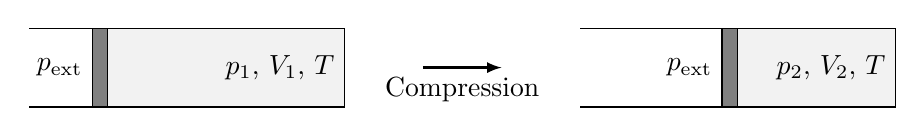
\begin{tikzpicture}
  %tikz thermo
    \fill[gray!10] (1, 0) rectangle (4,1);
    \draw[fill=gray] (1,0) rectangle (0.8, 1);
    \draw(0,0) -- (4,0) -- (4,1) -- (0,1);
    \draw (4,0.5) node[left]{$p_1$, $V_1$, $T$};
    \draw (0.8, 0.5) node[left]{$p_\text{ext}$ };

    \draw[thick, -latex] (5, 0.5) --node[below]{Compression} (6, 0.5);

    \begin{scope}[xshift=7cm]
    \fill[gray!10] (2, 0) rectangle (4,1);
    \draw[fill=gray] (2,0) rectangle (1.8, 1);
    \draw(0,0) -- (4,0) -- (4,1) -- (0,1);
    \draw (4,0.5) node[left]{$p_2$, $V_2$, $T$};
    \draw (1.8, 0.5) node[left]{$p_\text{ext}$ };
    \end{scope}
  \end{tikzpicture}
\end{center}
Comme la transformation est quasistatique, on a à chaque instant $p=p_\text{ext}$. Le gaz contenu dans le cylindre est supposé parfait, et donc on peut écrire la variation de son énergie interne comme 
\begin{equation}
  \Delta U = C_V \Delta T = 0
\end{equation}  
car la température reste constante au cours de la transformation. L'application du premier principe donne 
\begin{equation}
  \Delta U = W + Q = 0 \Leftrightarrow Q = -W
\end{equation}
pour déterminer l'échange de chaleur $Q$ avec le milieu extérieur, il suffit de calculer $W$ qui est le travail fourni au système par les forces de pression. On sait le calculer :
\begin{equation}
  W = -\int_{V_1}^{V_2} p_\text{ext} \D V = -\int_{V_1}^{V_2} p \D V = -\int_{V_1}^{V_2}\frac{nRT}{V}\D V
\end{equation}
On a utilisé l'équation d'état des gaz parfaits pour exprimer $p(V)$. Le calcul de l'intégrale donne 
\begin{equation}
  W = nRT\ln\left(\frac{V_1}{V_2}\right) = nRT \ln\left( \frac{p_2}{p_1} \right) > 0 \quad \text{car} \quad p_2>p_1
\end{equation}
et on a $Q = -W < 0$. On trouve, comme prévu, que le système reçoit de l'énergie sous forme de travail et fournit la même énergie sous forme de chaleur au milieu extérieur. 

On remarquera qu'on se trouve dans une situation où il y a un transfert thermique entre le système et le milieu extérieur alors que leurs températures sont identiques (le milieu extérieur est un thermostat à la température $T$).

\section{Enthalpie}%
\label{sec:enthalpie}

\subsection{Définition}%
\label{sub:definition_enthalpie}

On a vu que pour une transformation isochore, $\Delta U = Q + W_\text{autre}$, où $W_\text{autre}$ est le travail reçu qui n'est pas produit par les forces de pression. L'énergie interne est un fonction d'état bien adaptée pour étudier les transformations isochores, car si on connait l'expression de l'énergie interne d'un système en fonction de son état, on peut facilement calculer la chaleur qu'il échange avec l'extérieur lorsque $W_\text{autre}=0$. 

Nous allons montrer qu'il existe une autre fonction d'état appelée enthalpie et notée $H$ qui est bien adaptée à l'étude des transformations monobares.

Considérons un système globalement au repos, soumis à une transformation monobare, le premier principe donne 
\begin{equation}
  \Delta U = W + Q = W_\text{press} + W_\text{autre} + Q =  -p_\text{ext}\Delta V +  W_\text{autre} + Q = -\Delta(p_\text{ext}V) + W_\text{autre} + Q
\end{equation}
Comme l'état initial et l'état final de la transformation sont des états d'équilibre, ils sont à l'équilibre mécanique et $p=p_\text{ext}$. On peut dont écrire
\begin{equation}
  \Delta U = -\Delta(pV) + W_\text{autre} + Q
\end{equation}
ou encore
\begin{equation}
  \Delta(\underbrace{U+pV}_{H}) = W_\text{autre} + Q
\end{equation}
La quantité $U+pV$ est une fonction d'état car $U$ est une fonction d'état et $p$ et $V$ sont des variables d'état. On la note $H$ et on l'appelle enthalpie.

\begin{definition}
  L'enthalpie $H$ d'un système de volume $V$, pression $p$ et énergie interne $U$ est la fonction d'état 
  \begin{equation}
    H = U + pV
  \end{equation}
\end{definition}
Pour une transformation monobare où seules les forces de pression fournissent un travail, on a $\Delta H = Q$. L'enthalpie est une fonction d'état bien adaptée à l'étude des transformations monobares.

\subsection{Pour un gaz parfait}%
\label{sub:pour_un_gaz_parfait}
Nous allons déterminer l'expression de l'enthalpie d'un gaz parfait. D'après la définition de l'enthalpie, on a 
\begin{equation}
H = U + pV
\end{equation}
En utilisant l'équation d'état des gaz parfaits et l'expression de l'énergie interne d'un gaz parfait, on obtient
\begin{equation}
  H = C_V T + nRT = (\underbrace{C_V+nR}_{C_p})T = C_p T
\end{equation}
On trouve la \textbf{relation de Mayer} valable pour un gaz parfait :
\begin{eqencadre}
  C_p-C_V = nR
\end{eqencadre}
Où $C_p$ est la capacité thermique à pression constante du gaz. On aura donc toujours $C_p>C_V$. 


\subsection{Lois de Laplace}%
\label{sub:lois_de_laplace}
Lorsqu'un gaz parfait subit une évolution \textbf{quasistatique} et \textbf{adiabatique}, ses pression, volume et température sont reliés par les lois de Laplace.

Considérons une transformation adiabatique quasistatique d'un gaz parfait qui l'amène d'un volume $V_1$ et une pression $p_1 $ à un volume $V_2$ et une pression $p_2$ . On cherche une relation entre $p_1, V_1, p_2, V_2$. 

Pour cela, on décompose la transformation en une infinité de transformation \emph{élémentaires}. Lorsque le volume du gaz varie de $\D V$, le travail reçu est $\delta W = -p\D V$. Et l'application du premier principe à cette transformation élémentaire est
\begin{equation}
  \D U = C_V \D T = -p \D V
\end{equation}

car la chaleur $\delta Q$ reçue est nulle au cours de la transformation. En utilisant l'équation d'état des gaz parfaits pour exprimer $p$, on obtient
\begin{equation}
  C_V \D T = -\frac{nRT}{V}\D V \Leftrightarrow C_V \frac{\D T}{T} = -nR \frac{\D V}{V}
\end{equation}

On intègre l'équation précédente entre l'état initial et l'état final pour obtenir
\begin{equation}
  C_V\int_{T_1}^{T_2}\frac{\D T}{T} = -nR \int_{V_1}^{V_2}\frac{\D V}{V} \Leftrightarrow
  C_V\ln \left( \frac{T_2}{T_1} \right) = -nR\ln \left( \frac{V_2}{V_1} \right) = nR\ln \left( \frac{V_1}{V_2} \right)
\end{equation}
En utilisant la relation de Mayer $C_p-C_V=nR$ et en notant $\gamma=\frac{C_p}{C_v}$, on obtient
\begin{equation}
  (\gamma-1)\ln \left( \frac{V_1}{V_2} \right) = \ln \left( \frac{T_2}{T_1} \right) \Leftrightarrow T_1V_1^{\gamma-1} = T_2V_2^{\gamma-1}
\end{equation}
Et on a démontré que pour une transformation quasistatique adiabatique d'un gaz parfait
\begin{eqencadre}
  TV^{\gamma-1} = \text{constante}
\end{eqencadre}

En utilisant l'équation d'état des gaz parfaits, on montre aussi les deux autres lois de Laplace :
\begin{eqencadre}
  pV^\gamma = \text{constante} \quad \text{et} \quad T^\gamma p^{1-\gamma} = \text{constante}
\end{eqencadre}


\subsection{Pour une phase condensée incompressible et indilatable}%
\label{sub:pour_une_phase_condensee_incompressible_et_indilatable}

On a déjà vu que l'énergie interne d'une phase condensée incompressible, indilatable ne dépend que de sa température. On admettra qu'il en est de même pour l'enthalpie, et que pour une phase condensée incompressible, indilatable l'enthalpie est égale à l'énergie interne et donc
\begin{eqencadre}
  H(T) = U(T) = C_V T = C_p T = C T
\end{eqencadre}
La capacité thermique à volume constant est égale à la capacité thermique à pression constante (appelée simplement \emph{capacité thermique}).

Par exemple, pour l'eau liquide, la capacité thermique molaire à volume constant est $C_{Vm}\approx \SI{75}{\joule\per\mole}$ et le volume molaire est $V_m\approx \SI{2e-5}{\cubic\meter\per\mol}$. Si l'eau liquide subit une transformation pour laquelle $\Delta T = \SI{1}{K}$  et $\Delta p = \SI{1}{\bar}$, on aura la variation d'enthalpie molaire :
\begin{equation}
  \Delta H_m = \underbrace{\Delta U_m}_{\approx \SI{75}{\joule\per\mole}} + \underbrace{V_m\Delta P}_{\approx \SI{2}{\joule\per\mole}} \approx \Delta U_m = C_{Vm} \Delta T
\end{equation}

\subsection{Application}%
\label{sub:application_enthalpie}

On chauffe \SI{1}{\litre} d'eau initialement à \SI{20}{\celsius} dans une bouilloire dont les parois sont calorifugées (pas de transfert thermique) de puissance $P=\SI{2000}{\watt}$. Calculer le temps mis pour faire bouillir l'eau. On donne $c_\text{eau}=\SI{4.2}{\joule\per\gram\per\kelvin}$.  

Lorsque l'eau est chauffée dans la bouilloire, c'est une transformation monobare, car la pression extérieure est la pression atmosphérique qui est constante. On a donc d'après le premier principe
\begin{equation}
  \Delta H = Q + W_\text{autre} = C_p \Delta T = m_\text{eau} c_\text{eau} \Delta T
\end{equation}
Or $Q=0$ car les parois de la bouilloire sont calorifugées et $W_\text{autre}$ correspond à l'énergie électrique reçue par la bouilloire et vaut $W_\text{autre}=Pt$ 

On obtient donc 
\luaexec{P=2e3; m=1e3; c=4.2; T1=20; T2=100}
\begin{equation}
  t =\frac{m_\text{eau}c_\text{eau}\Delta T}{P}\approx \luaexec{SI(m*c*(T2-T1)/P, 0, "\\second")}
\end{equation}
En pratique les parois ne sont pas parfaitement isolées thermiquement, $Q<0$ et $t$ est un peu plus grand.

\section{Enthalpie de changement d'état}%
\label{sec:enthalpie_de_changement_d_etat}

\subsection{Définition}%
\label{sub:definition_enthalpie_chgt_etat}

L'enthalpie de changement d'état est la variation d'enthalpie d'un corps pur lorsqu'il change d'état à $p$ et $T$ constants. 

\begin{center}
\begin{tikzpicture}
  \begin{axis}[
  xmode=log,
  ymin=0,
  ymax=1.5,
  width=11cm,
  height=8cm,
  xlabel near ticks,
  ylabel near ticks,
  xmin=0.3,
  xticklabels={},
  yticklabels={},
  xlabel = Volume massique $v$,
  ylabel = Pression $p$, 
  extra y ticks={0.09,1},
  extra y tick labels={$p_T$, $p_C$}, 
  ]
   \addplot[mark=none, smooth, gray, thin] table[x index=0, y index=3] {data/isothermes.csv};
    
    \draw[dashed, gray] (axis cs:0.01, 1) -- (axis cs:25,1);
    \draw[dashed, gray] (axis cs:0.01, 0.09) -- (axis cs:25,0.09);
    \addplot[mark=none, thick] table[x index=0, y index=2] {data/clapeyron.csv};
    \addplot[mark=none, thick] table[x index=1, y index=2] {data/clapeyron.csv};
    \draw[fill=black] (axis cs:1,1) circle(2pt) node[above]{$C$};
    
    \coordinate (A) at (axis cs:0.518, 0.383362);
    \coordinate (B) at (axis cs:4.197, 0.383362);
    \coordinate (M) at (axis cs:2, 0.383362);

    \fill (A) circle(2pt) node[left]{$A$};
    \fill (B) circle(2pt) node[right]{$B$};
  \end{axis}
  \end{tikzpicture}
  \end{center}
  Sur le diagramme de Clapeyron ci-dessus, l'enthalpie de vaporisation $H_v$  correspond à la variation d'enthalpie entre les points $A$ (liquide) et $B$ (gaz). 
  \begin{equation}
    H_v = H(B) - H(A)
  \end{equation}
  on définit les enthalpies de vaporisation $H_v$, de fusion $H_f$ et de sublimation $H_s$. 

  Remarques :
  \begin{itemize}
    \item On donne généralement les enthalpies massiques de changement d'état $h_v$, $h_f$, et $h_s$. 
    \item Une enthalpie de changement d'état correspond à une différence d'enthalpies : $h_v = h_\text{gaz} - h_\text{liquide}$ 
  \end{itemize}
  \subsection{Application}%
  \label{sub:application_enthalpie_chgt_etat}
  On chauffe dans une bouilloire de $P=\SI{2000}{\watt}$, $m=\SI{1}{\kilo\gram}$ de glace initialement à $T_1=\SI{-20}{\celsius}$. Déterminer le temps nécessaire pour faire bouillir l'eau.

  On applique comme dans la partie précédente le premier principe et on décompose l'évolution du système en plusieurs étapes :
  \begin{equation}
    \Delta H = W_\text{elec} = \Delta H_\text{glace} + H_\text{fusion} + \Delta H_\text{liquide}
  \end{equation}

  avec $\Delta H_\text{glace}=mc_\text{glace}\Delta T_\text{glace}$ ; $H_\text{fusion}=mh_f$ ; $\Delta H_\text{liquide}=mc_\text{liquide}\Delta T_\text{liquide}$ ; 

  et 
  $\Delta T_\text{liquide} = \SI{100}{\kelvin}$ ; $\Delta T_\text{glace} = \SI{20}{\kelvin}$ ; $h_f = \SI{333}{\joule\per\gram}$ ; $c_\text{liquide}=\SI{4.18}{\joule\per\gram\per\kelvin}$ ; $c_\text{glace} = \SI{2.06}{\joule\per\gram\per\kelvin}$. 
  \luaexec{cl=4.18; cg=2.06; m=1e3; dTg=20; dTl=100; hf=333; P=2e3}
  On trouve 
  \begin{equation}
    t= \frac{mc_\text{liquide}\Delta T_\text{liquide}+mc_\text{glace}\Delta T_\text{glace}+mh_f}{P}\approx\luaexec{SI((cl*dTl*m+cg*dTg*m+hf*m)/P, 0, "\\second")}
  \end{equation}
  
  
\end{document}
